\Chapter{Power Supply Design and Modelling}
\label{chap:modelling}
Power supply for the WEDM process delivers intermittent current and voltages across the electrode-dielectric-silicon ingot assembly. The pulsed nature of this power supply makes the design for such circuit difficult. This chapter describes the working of an ideal power source for the WEDM process followed by its converter topology. The linear and nonlinear models are then derived for this converter.

\section{Working Principle}
	Figure \ref{fig:working-1} represents the functional configuration of a pulsed power supply in which an ideal current source $I_o$ and ideal voltage source $V_o$ are connected in parallel across the spark gap load $E$. The current and voltage waveforms across the load are shown in figure \ref{fig:working-2}
	\begin{figure}[H]
		\begin{subfigure}{0.49\textwidth}
			\vspace{0.5cm}
			\centering
			\includegraphics[width=\linewidth]{rep-diag-master}
			\caption{Representative diagram}
			\label{fig:working-1}
		\end{subfigure}
		\begin{subfigure}{0.49\textwidth}
			\centering
			\includegraphics[width=\linewidth]{working-wf-master}
			\caption{Load voltage and current}
			\label{fig:working-2}
		\end{subfigure}
		\caption{Working of WEDM supply}
	\end{figure}

\subsection{Pre-Breakdown}
	During times $t=t_0$ and $t=t_1$, the current source causes the diode $D$ to turn on and $I_o$ flows through $D$ to the ideal voltage source $V_o$. The voltage across the load terminals is $V_o$ because $D$ remains in a conduction state from $t_0$ to $t_1$. This application of voltage across the spark gap terminals causes the gap to break down at $t=t_1$. This breakdown delay time depends on the dielectric strength and the magnitude of the applied voltage.
	\begin{figure}[H]
		\centering
		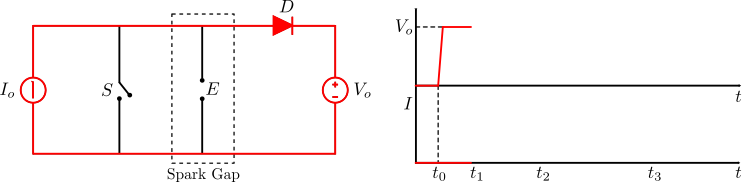
\includegraphics[width=\textwidth]{working-1}
		\caption{Pre-breakdown stage}
		\label{fig:working-1}
	\end{figure}

\subsection{Sparking}
	Due to breakdown of dielectric, current $I_o$ starts flowing through the spark gap $E$ and the diode $D$ turns off. If the spark gap is modelled as a resistance, the voltage across terminals is $V_{dis}$ and is equal to $I_or_{gap}$. The silicon ingot now erodes along the length of moving wire electrode.
	\begin{figure}[H]
		\centering
		\includegraphics[width=\textwidth]{working-2}
		\caption{Sparking stage}
		\label{fig:working-2}
	\end{figure}	

\subsection{Dead Time}
	The \emph{dead} time zone serves three purposes: (a) avoids a sustained arc (and hence a short circuit) (b) gives time for removal of debris from the gap and (c) allows the tool electrode to move closer to the workpiece. This is achieved closing the switch $S$ at time $t=t_2$. When $S$ is closed, the current $I_o$ flows through current source and switch and dielectric strength of the medium is recovered by flushing fresh dielectric over the gap.
	\begin{figure}[H]
		\centering
		\includegraphics[width=\textwidth]{working-3}
		\caption{Dead time stage}
		\label{fig:working-3}
	\end{figure}
	When the gap is fully recovered, a new machining cycle is started at time $t=t_3$ by opening the switch $S$. The erosion takes place for about 10\% of the entire machining period. Thus, the power is supplied to load only for this fraction of the machining period.

\section{Converter Topology}
	\begin{figure}[h]
		\centering
		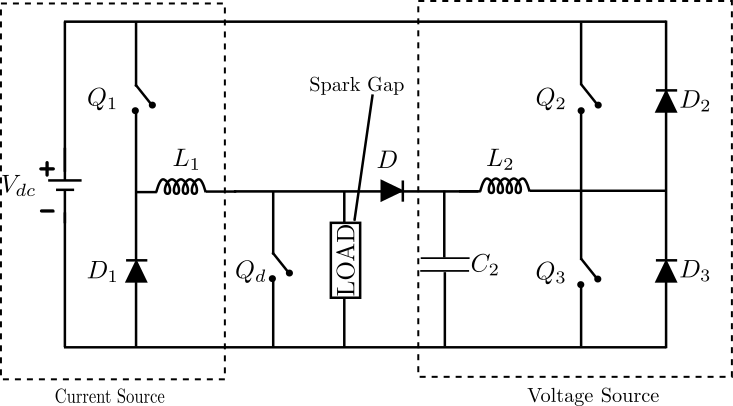
\includegraphics[width=0.9\textwidth]{conv-top-master}
		\caption{Converter topology for WEDM power supply}
		\label{fig:working-3}
	\end{figure}
	This section describes the practical implementation of the ideal current and voltage sources depicted in figure \ref{fig:working-1}. One realisation of such power supply is proposed by Tastekin et al. in \cite{tastekin2009novel} in which a single quadrant and a two quadrant DC-DC converter is connected to the same DC link. A single quadrant converter is used as current source by controlling the inductor current and removing the filter capacitance. The voltage source is realised by controlling the output voltage of the two quadrant converter. Figure \ref{fig:working-3} depicts this configuration using high frequency power electronic switches.

	Constant voltage of $V_o$ is maintained at the load terminals of the two quadrant converter. However, when switch $S$ in figure \ref{fig:working-1} is opened, the current $I_o$ goes through $D$ to the capacitor of the two quadrant converter. This acts as a disturbance to the voltage source controller and must be rejected at the earliest to maintain the constant voltage across the load terminals.

	This implementation does not use transistors and resistors, hence the only losses incurred are the switching and conduction losses of the power electronic switches, and the inductor copper losses.
	
\section{Linear Modelling}
	%The power supply depicted in figure \ref{fig:working-3} is composed of three components viz. single quadrant converter acting as current source, two quadrant converter acting as voltage source, and the ignition switch. 
	A controller is required to regulate the current of the quadrant converter and the voltage of the the two quadrant converters each, hence the state space model for these converters is found out. This section explains the time averaging method to arrive at the small signal models between the output voltage or current and the duty ratio of the switches for both the converters.

\subsection{Voltage Source}
	\begin{figure}[H]
		\begin{subfigure}{0.49\textwidth}
			\centering
			\includegraphics[width=\linewidth]{2quad-mod-master}
			\caption{Modified}
			\label{fig:working-4}
		\end{subfigure}
		\begin{subfigure}{0.49\textwidth}
			\centering
			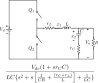
\includegraphics[width=\linewidth]{2quad_norm}
			\caption{Standard}
			\label{fig:working-4b}
		\end{subfigure}
		\caption{Simplified circuit of two quadrant converter}
		\label{fig:2quad-comparison}
	\end{figure}
	Figure \ref{fig:working-4} represents the simplified circuit for the two quadrant converter which is to be, hence the small signal transfer function $\dfrac{\hat{v}_o}{\hat{d}}$ is to be found out. The current through the inductor $L$ and the voltage across capacitor $C$ are considered as the state variables.

	When the switch $Q_2$ is on i.e. for time $DT_s$, current flows though $V_d$, $Q_2$, $r_{L}$, $L$, $r_{C}$ and $C$. Applying Kirchhoff's Voltage Law along this path gives
	\begin{equation}
		V_d - L \dot{x}_1 - r_{L}x_1 - r_{C}x_1-x_2 = 0
		\label{eq:mod1}
	\end{equation}
	From current through the inductor and the capacitor is same, therefore
	\begin{equation}
		x_1 = C\dot{x_2} 
		\label{eq:mod2}
	\end{equation}
	The output voltage is
	\begin{equation}
		V_o = r_{C}x_1 + x_2
		\label{eq:mod3}
	\end{equation}
	\begin{equation}
		\begin{split}
		\therefore \dot{x}_1 &= -\dfrac{r_{L}+r_{C}}{L}x_1 -\dfrac{1}{L}x_2+\dfrac{1}{L}V_d\\
		\dot{x}_2 &= \dfrac{1}{C}x_1\\
		V_o &= r_{C}x_1 + x_2
		\end{split}
		\label{eq:mod4}
	\end{equation}
	When $Q_2$ is off i.e. for time $(1-D)T_s$, current flows through  $D_3$, $r_{L}$, $L$, $r_{C}$ and $C$. Applying Kirchhoff's Voltage Law along this path gives
	\begin{equation}
		- L \dot{x}_1 - r_{L}x_1 - r_{C}x_1-x_2 = 0
		\label{eq:mod5}
	\end{equation}
	Also,
	\begin{equation}
		x_1 = C\dot{x_2} 
		\label{eq:mod6}
	\end{equation}
	The output voltage is
	\begin{equation}
		V_o = r_{C}x_1 + x_2
		\label{eq:mod7}
	\end{equation}
	\begin{equation}
		\begin{split}
			\therefore \dot{x}_1 &= -\dfrac{r_{L}+r_{C}}{L}x_1 -\dfrac{1}{L}x_2\\
			\dot{x}_2 &= \dfrac{1}{C}x_1\\
			V_o &= r_{C}x_1 + x_1
		\end{split}
		\label{eq:mod8}
	\end{equation}
	Constructing the state vector $x$ as
	\begin{equation}
		x =
		\begin{bmatrix}
			x_1\\x_2
		\end{bmatrix}
		\label{eq:mod9}
	\end{equation}
	In equation \eqref{eq:4}, let
	\begin{equation}
		A_1=
		\begin{bmatrix}
			-\dfrac{r_{L}+r_{C}}{L} & -\dfrac{1}{L}\vspace*{2mm}\\
			\dfrac{1}{C} & 0
		\end{bmatrix}
		\quad
		B_1=
		\begin{bmatrix}
			\dfrac{1}{L} \vspace*{2mm}\\ 0
		\end{bmatrix}
		\quad
		C_1 =
		\begin{bmatrix}
			r_{C} & 1
		\end{bmatrix}
		\label{eq:mod10}
	\end{equation}
	\begin{equation}
		\begin{split}
			\therefore \dot{x} &= A_1 x + B_1 V_d\\
			V_o &= C_1 x
		\end{split}
		\label{eq:mod11}
	\end{equation}
	In equation \eqref{eq:5}, let
	\begin{equation}
		A_2=
		\begin{bmatrix}
			-\dfrac{r_{L}+r_{C}}{L} & -\dfrac{1}{L}\vspace*{2mm}\\
			\dfrac{1}{C} & 0
		\end{bmatrix}
		\quad
		B_2=
		\begin{bmatrix}
			0 \vspace*{2mm}\\ 0
		\end{bmatrix}
		\quad
		C_1 =
		\begin{bmatrix}
			r_{C} & 1
		\end{bmatrix}
		\label{eq:mod12}
	\end{equation}
	\begin{equation}
		\begin{split}
			\therefore \dot{x} &= A_1 x + B_1 V_d\\
			V_o &= C_1 x
		\end{split}
		\label{eq:mod13}
	\end{equation}
	Equation \eqref{eq:mod11} is valid for $dT_s$ and equation \eqref{eq:mod13} is valid for $(1-d)T_s$. Time averaging equations \eqref{eq:mod11} and \eqref{eq:mod13} leads to
	\begin{equation}
	    \begin{split}
    		\dot{x} &= [dA_1+(1-d)A_2]x + [dB_1 + (1-d)B_2]V_d\\
	    	V_o &= [dC_1+(1-d)C_2]x
		    \label{eq:mod14}
	    \end{split}
	\end{equation}

	Small signal transfer function for this representation is derived by introducing small perturbations in $x$, $V_o$, and $d$ and eliminating the steady state quantities. Complete mathematical treatment is described in pp.324-325 of \citet{book:768263}. The small signal transfer function of the output voltage of two quadrant converter with respect to the duty ratio of the switch $Q_2$ turns out to be \cite{book:768263}
	\begin{equation}
		\therefore \dfrac{\hat{v}_o(s)}{\hat{d}(s)} = C[sI-A]^{-1}[(A_1-A_2)X+(B_1-B_2)V_d]+(C_1-C_2)X
		\label{eq:mod27a}
	\end{equation}
	The scalar form of this transfer function is shown in table \ref{tab:vstf}.
	\begin{table}[h]
	\centering
	\begin{tabular}{|p{6cm}|p{8cm}|} \hline
	\multicolumn{1}{|c|}{Modified} & \multicolumn{1}{c|}{Standard} \\ \hline
	\vspace{-2mm} \(\displaystyle \dfrac{\hat{v}_o(s)}{\hat{d}(s)} = \dfrac{V_{dc}(Cr_Cs+1)}{LCs^2+(Cr_C+Cr_L)s+1} \) & \vspace{-2mm} \(\displaystyle \dfrac{\hat{v}_o(s)}{\hat{d}(s)} = \dfrac{V_{dc}(Cr_Cs+1)}{LC\{s^2+s\left[\dfrac{1}{RC} + \dfrac{(r_C + r_L)}{L} \right]+\dfrac{1}{LC}\}}\) \vspace{1mm} \\ \hline
	\end{tabular}
	\caption{Scalar transfer function of voltage source}
	\label{tab:vstf}
	\end{table}
	
	The bode plot for this transfer function when the values of inductors and capacitors are chosen as described in chapter \ref{chap:hardware} is shown in figure \ref{fig:uncomp-vs}
	\begin{comment}
		\begin{figure}[h]
			\centering
			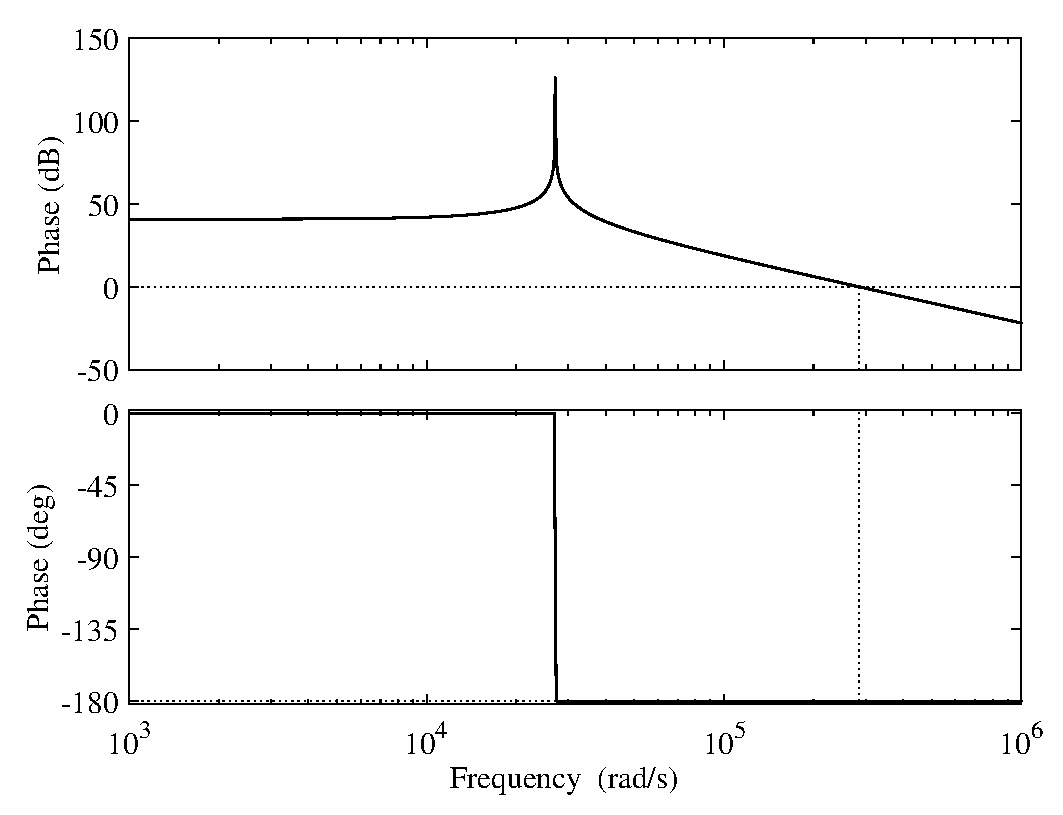
\includegraphics[width=0.8\textwidth]{uncompensated-vs}
			\caption{Bode plot of uncompensated transfer function of voltage source; Gm = $\infty$,  Pm = 0.0166$^\circ$ (at 2.85e+05 rad/s)}
			\label{fig:uncomp-vs}
		\end{figure}
	\end{comment}
	\begin{figure}[H]
		\centering
		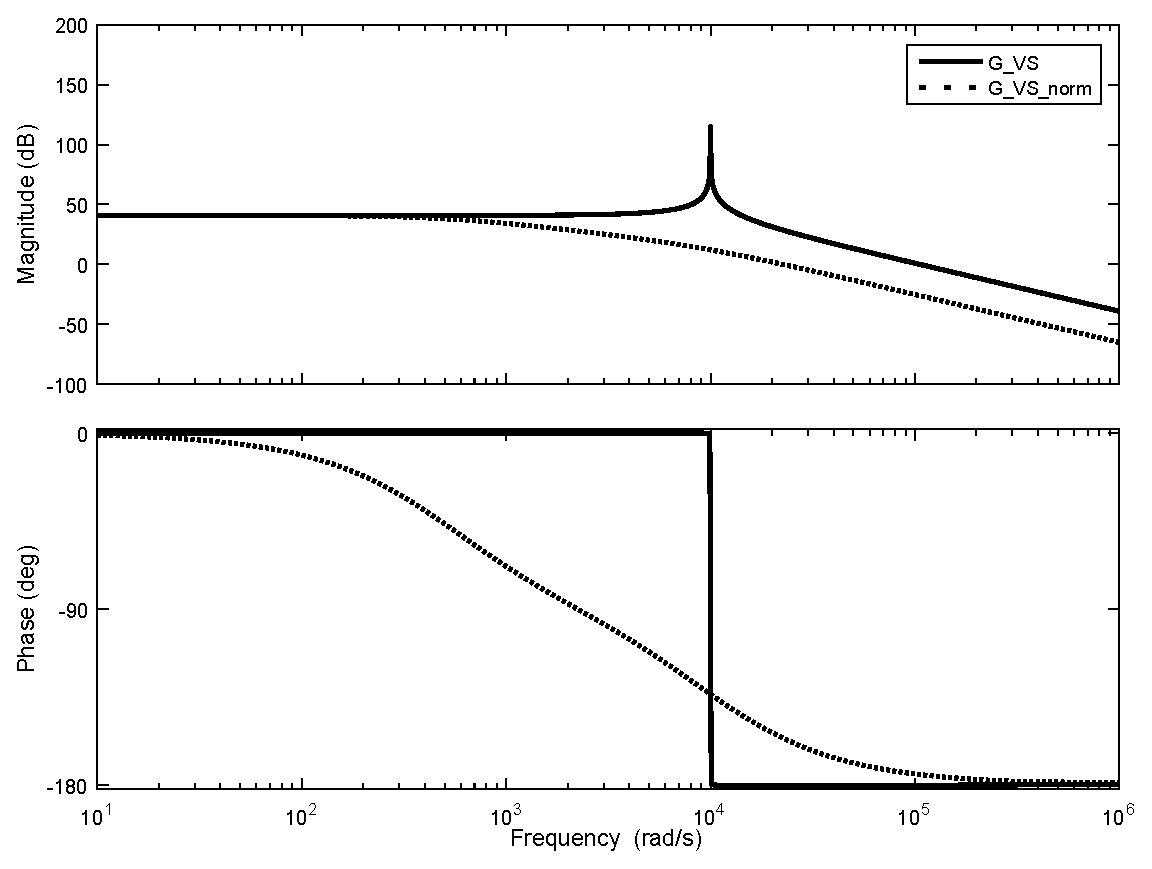
\includegraphics[width=0.7\textwidth]{vs_comparison}
		\caption{Bode plot of voltage source}
		\label{fig:uncomp-vs}
	\end{figure}
	The magnitude of peak in the bode plot of the modified two quadrant converter is more as compared to that of the standard counterpart. The removal of the resistance from the output of the standard two quadrant converter causes reduction in the damping factor which is observable in figure \ref{fig:uncomp-vs}.

\subsection{Current Source}
	\begin{figure}[H]
		\begin{subfigure}{0.49\textwidth}
			\centering
			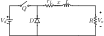
\includegraphics[width=\linewidth]{buck-mod-master}
			\caption{Modified}
			\label{fig:working-5}
		\end{subfigure}
		\begin{subfigure}{0.49\textwidth}
			\centering
			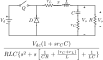
\includegraphics[width=\linewidth]{buck_norm}
			\caption{Standard}
			\label{fig:working-5b}
		\end{subfigure}
		\caption{Simplified circuit of single quadrant converter}
		\label{fig:buck-comparison}
	\end{figure}
	Similar approach is applied for finding out the transfer function of the output current with respect or the duty cycle of the switch $Q_1$ for the single quadrant converter. Figure \ref{fig:working-5} shows the simplified circuit diagram for the same. The current through the inductor $L$ is the only state variable in this case.

	When the switch $Q_1$ is on i.e. for time $dT_s$, current flows though $V_d$, $Q_1$, $r_{L}$, $L$ and $R_L$. Applying Kirchhoff's Voltage Law along this path gives
	\begin{equation}
		V_d - L \dot{x} - r_{L}x - R_Lx = 0
		\label{eq:mod28}
	\end{equation}
		The output current is
	\begin{equation}
		I_o = x
		\label{eq:mod29}
	\end{equation}
	\begin{equation}
		\begin{split}
			\therefore \dot{x} &= -\dfrac{r_{L}+R_L}{L}x +\dfrac{1}{L}V_d\\
			I_o &= x	
		\end{split}
		\label{eq:mod30}
	\end{equation}
	When $Q_1$ is off i.e. for time $(1-d)T_s$, current flows through  $D_1$, $r_{L}$, $L$ and $R_L$. Applying Kirchhoff's Voltage Law along this path gives
	\begin{equation}
		- L \dot{x} - r_{L}x - R_Lx = 0
		\label{eq:mod31}
	\end{equation}
	The output current is
	\begin{equation}
		I_o = x
		\label{eq:mod32}
	\end{equation}
	\begin{equation}
		\begin{split}
			\therefore \dot{x} &= -\dfrac{r_{L}+R_L}{L}x\\
			I_o &= x
		\end{split}
		\label{eq:mod33}
	\end{equation}
	\begin{equation}
		\begin{split}
			\therefore A_1 &= -\dfrac{r_{L}+R_L}{L} = A_2\\
			B_1 &= \dfrac{1}{L} \quad B_2 = 0\\
			C_1 &= 1 = C_2
		\end{split}
		\label{eq:mod34}
	\end{equation}
	The transfer function $\dfrac{\hat{i}_o}{\hat{d}}$ is obtained using equations \eqref{eq:mod34} in following \cite{book:768263} 
	\begin{equation}
		\dfrac{\hat{i}_o(s)}{\hat{d}(s)} = C[sI-A]^{-1}[(A_1-A_2)X+(B_1-B_2)V_d]+(C_1-C_2)X
		\label{eq:mod35}
	\end{equation}
	where
	\begin{align}
		A &= A_1d+A_2(1-d)
		\label{eq:mod36}
	\end{align}
		The scalar form of this transfer function is shown in table \ref{tab:cstf}.
	\begin{table}[h]
	\centering
	\begin{tabular}{|p{4cm}|p{8cm}|} \hline
	\multicolumn{1}{|c|}{Modified} & \multicolumn{1}{c|}{Standard} \\ \hline
	\vspace{-2mm} \(\displaystyle \dfrac{\hat{i}_o(s)}{\hat{d}(s)} = \dfrac{V_{dc}}{(R+r_L)+Ls} \) & \vspace{-2mm} \(\displaystyle \dfrac{\hat{i}_o(s)}{\hat{d}(s)} = \dfrac{V_{dc}(Cr_Cs+1)}{RLC\{s^2+s\left[\dfrac{1}{RC} + \dfrac{(r_C + r_L)}{L} \right]+\dfrac{1}{LC}\}}\) \vspace{1mm} \\ \hline
	\end{tabular}
	\caption{Scalar transfer function of current source}
	\label{tab:cstf}
	\end{table}

	The bode plot for this transfer function when the values of inductors and capacitors are chosen as described in \ref{chap:hardware} is shown in figure \ref{fig:uncomp-cs}
	\begin{comment}
		\begin{figure}[H]
			\centering
			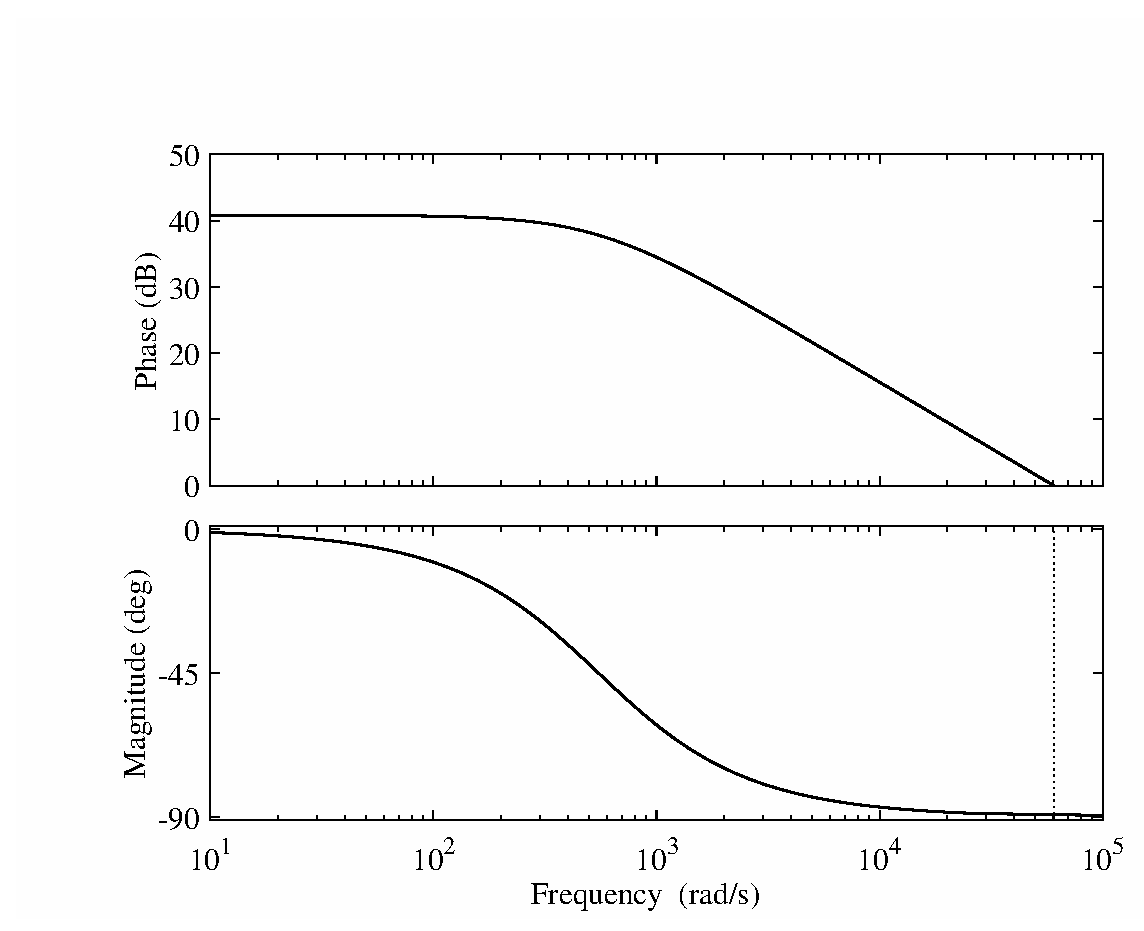
\includegraphics[width=0.8\textwidth]{uncompensated-cs}
			\caption{Bode plot of uncompensated current source transfer function; Gm = $\infty$,  Pm = 90.5$^\circ$ (at 6.05e+04 rad/s)}
			\label{fig:uncomp-cs}
		\end{figure}
	\end{comment}
	\begin{figure}[h]
		\centering
		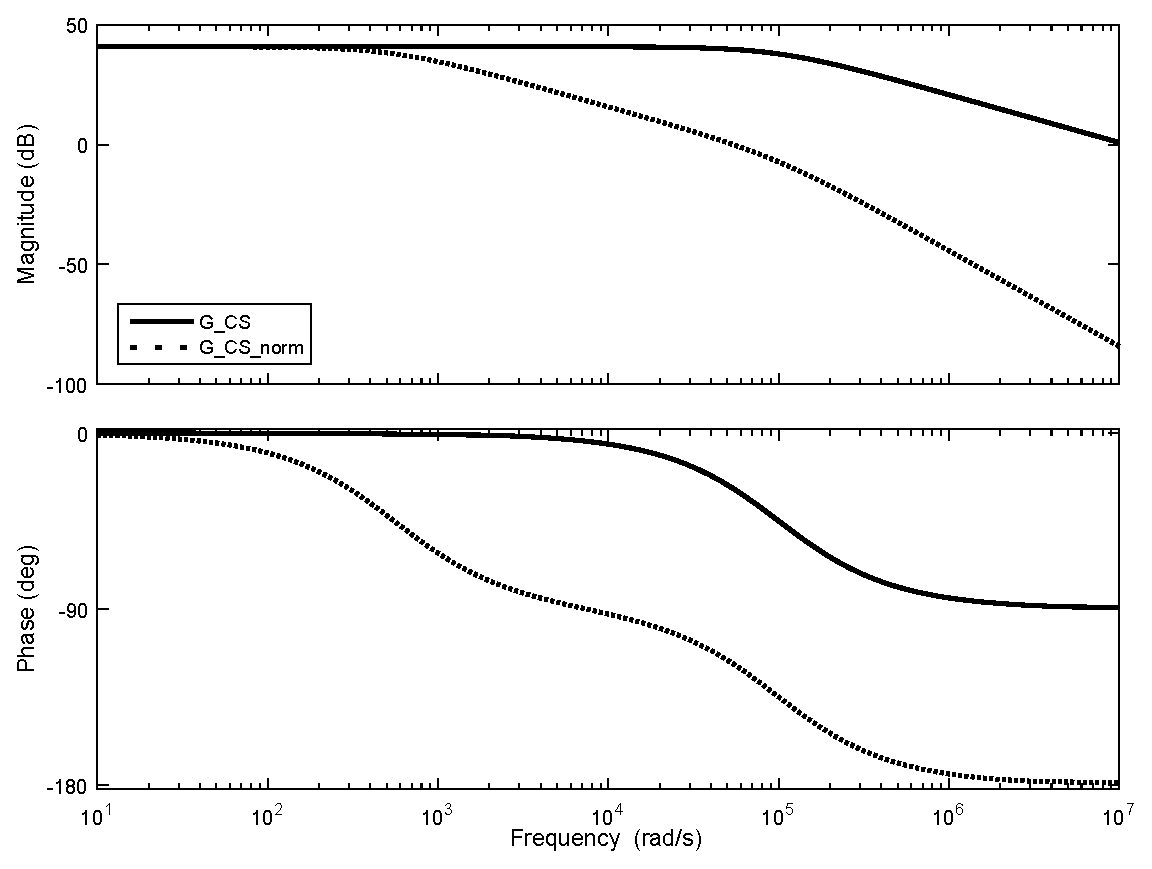
\includegraphics[width=0.8\textwidth]{cs_comparison}
		\caption{Bode plot of current source}
		\label{fig:uncomp-cs}
	\end{figure}
	Due to the removal of the output capacitor in the standard buck converter, the order of the system is reduced to one.
	
\section{Nonlinear Modelling}
	The approach described in the previous section relies on the approximation of switching phenomenon by duty ratio. Hence, a nonlinear model is derived for current and voltage sources based on the phase plane analysis.
	\subsection{Voltage Source Model}
    Figure \ref{fig:nl-1} depicts simplified two quadrant converter which constitutes the voltage source in the pulsed power topology. The resistances of inductor and capacitor shown are ignored for simplified mathematical treatment. To derive a nonlinear model of this converter, following choices of state variables are made.
    \begin{align*}
    	x_1 &= v - v_{ref} \\
    	x_2 &= \dot{x_1} = \frac{i_C}{C}
    \end{align*}
    Let the switch state if $Q_1$ be the input $u$ such that $Q_1$ is ON when $u = 1$ and OFF when $u = 0$. $Q_2$ is complementary to $Q_1$, hence, $Q_2$ is OFF when $u = 1$ and ON when $u = 0$. Applying Kirchhoff's Voltage Law for both the circuit states
    \begin{align*}
        u &= 1 \implies \dot{x_2} = -\frac{x_1}{LC} -\frac{V_{ref}}{LC} + \frac{V_{dc}}{LC}\\
        u &= 0 \implies \dot{x_2} = -\frac{x_1}{LC} -\frac{V_{ref}}{LC}
    \end{align*}
    Thus, the complete dynamics of the voltage source are
    \begin{align}
        \dot{x_1} &= x_2\\
        \dot{x_2} &= -\frac{x_1}{LC} + u\frac{V_{dc}}{LC} -\frac{V_{ref}}{LC}
        \label{eq:nl1}
    \end{align}
	\begin{figure}[h]
		\begin{subfigure}{.55\textwidth}
          \centering
          \includegraphics[width=0.9\linewidth]{nl-2quad-mod-master}
          \caption{Two quadrant converter}
          \label{fig:nl-1}
        \end{subfigure}
        \begin{subfigure}{.4\textwidth}
          \vspace{2cm}
          \centering
          \includegraphics[width=0.9\linewidth]{nl-buck-mod-master}
          \caption{Single quadrant converter}
          \label{fig:nl-2}
        \end{subfigure}
		\caption{Nonlinear modelling circuit}
	\end{figure}

\subsection{Current Source Model}
    Figure \ref{fig:nl-2} shows simplified single quadrant converter which constitutes the current source in the pulsed power topology. To derive a nonlinear model of this converter, the state variable is chosen as
    \begin{align*}
    	x_1 = i - i_{ref}
    \end{align*}
    Let the switch state of $Q$ be the input $u$ such that $Q$ is ON when $u = 1$ and OFF when $u = 0$. Applying Kirchhoff's Voltage Law for both the circuit states
    \begin{align*}
        u &= 1 \implies \dot{x_1} = -\frac{R}{L}x_1 -\frac{R}{L}i_{ref} + \frac{V_{dc}}{L}\\
        u &= 0 \implies \dot{x_1} = -\frac{R}{L}x_1 -\frac{R}{L}i_{ref}
    \end{align*}
    Thus, the complete dynamics of the current source are
    \begin{align}
        \dot{x_1} &= -\frac{R}{L}x_1 + u\frac{V_{dc}}{L} -\frac{R}{L}i_{ref}
        \label{eq:nl2}
    \end{align}